\documentclass[a4paper]{article}

% ===== Packages =====
\usepackage[T1]{fontenc}        % Font encoding
\usepackage{lmodern}
\usepackage{algorithm}
\usepackage{subcaption}

% Modern font
\usepackage[a4paper,margin=0.8in]{geometry} % Page layout: 1in margin
\usepackage[fleqn]{amsmath}     % Math symbols, left-aligned equations
\setlength{\mathindent}{0pt}    % No indent for fleqn
\usepackage{amssymb}            % Extra math symbols
\usepackage{booktabs}           % Better tables
\usepackage{graphicx}           % Include graphics
\usepackage{setspace}           % Adjust line spacing
\usepackage{titling}            % Customize title format
\usepackage{float}              % [H] for figure placement
\usepackage{color}              % For colored text
\usepackage{booktabs}           % For better tables

\usepackage{algorithm}
\usepackage{algorithmic}
\renewcommand{\thealgorithm}{\arabic{algorithm}} % Numerazione autonoma

\newcommand{\todo}[1]{\textcolor{red}{\textbf{TODO:} #1}}

% ===== Line spacing =====
\setstretch{0.9}                % 0.9× spacing; regola a piacere

% ===== Title formatting =====
\pretitle{%
  \begin{center}\bfseries\Large
  }
  \posttitle{%
  \end{center}\vspace{-1em}
}
\preauthor{%
  \begin{center}\small
  }
  \postauthor{%
  \end{center}\vspace{-1em}
}
\predate{}  % no date before
\postdate{} % no date after

% ===== Metadata =====
\title{Report HW2}
\author{%
  \ifdefined\anonymous%
  Anonymous Submission
  \else
  \begin{tabular}{cc}
    Simone De Carli & Damiano Salvaterra \\
    {\small\texttt{simone.decarli@studenti.unitn.it}} &
    {\small\texttt{damiano.salvaterra@studenti.unitn.it}}
  \end{tabular}
  \fi
}
\date{}  % leave date blank

\begin{document}

\maketitle

\section*{Exercise 1}

We aim to simulate a Poisson process with a fixed number of arrivals
$N$. Given the time interval $[0, T]$, with $T = 100$ the rate
parameter is set as $\lambda = \frac{N}{T}$.

\subsection*{Part 1: Uniform Arrival Times}

In this experiment, we generate $k$ realizations of $N$ arrival times
sampled uniformly over $[0, T]$. Then we sort them to compute the
inter-arrival times.
We aggregate the inter-arrival times from all $k$ to assess whether
they follow an exponential distribution. Specifically, we:

\begin{itemize}
    \setlength\itemsep{0.01em}
  \item Plot the histogram of all inter-arrival times across the $k$
    realizations, overlaid with the corresponding exponential
    probability density function (PDF), as shown in
    Figure~\ref{fig:ex1-p1-combined}.
  \item Construct a Q-Q plot comparing the empirical distribution of
    inter-arrival times with the theoretical exponential distribution
    (Figure~\ref{fig:ex1-p1-combined}).
  \item Compute empirical mean and variance, and compare them to
    theoretical values. (Table~\ref{tab:ex1-p1-ci-summary}).
\end{itemize}

\begin{table}[htbp]
  \centering
  \small
  \begin{tabular}{@{}cc|lcccccc@{}}
    \toprule
    $\lambda$ & $k$ & Source & Mean & Var & Mean 95\% CI & Mean 99\%
    CI & Var 95\% CI & Var 99\% CI \\
    \midrule
    100 & $10^3$ & Theoretical & 0.01 & 0.00 & -- & -- & -- & -- \\
    100 & $10^3$ & Empirical   & 0.01 & 0.00 & [0.01,0.01] &
    [0.01,0.01] & [0.00,0.00] & [0.00,0.00] \\
    \midrule
    0.42 & $10^6$ & Theoretical & 2.38 & 5.67 & -- & -- & -- & -- \\
    0.42 & $10^6$ & Empirical   & 2.33 & 5.16 & [2.32,2.33] &
    [2.32,2.33] & [5.14,5.19] & [5.13,5.20] \\
    \bottomrule
  \end{tabular}
  \caption{Summary of inter-arrival time statistics: mean, variance,
    and confidence intervals for both experimental
  setups.}\label{tab:ex1-p1-ci-summary}
\end{table}

\begin{figure}[htbp]
  \centering
  \begin{subfigure}[b]{0.48\textwidth}
    \centering
    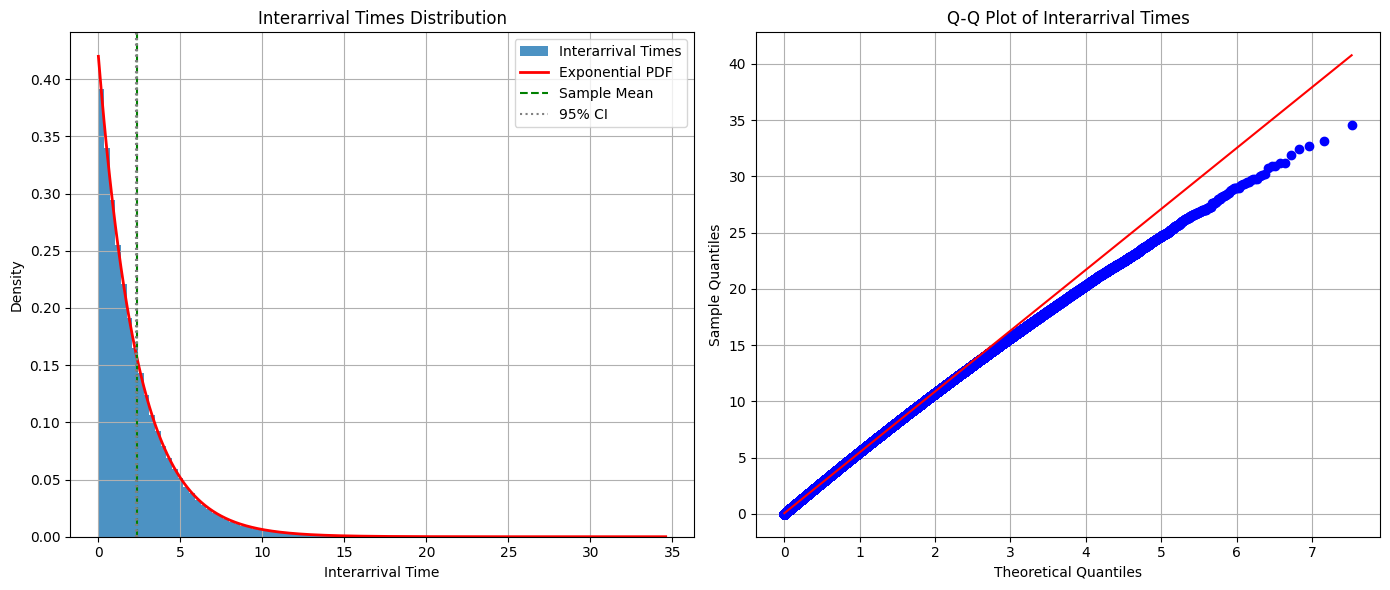
\includegraphics[width=\textwidth]{images/ex1-p1.png}
    \caption{$k = 10^6$ and $\lambda = 0,42$.}\label{fig:ex1-p1}
  \end{subfigure}
  \hfill
  \begin{subfigure}[b]{0.48\textwidth}
    \centering
    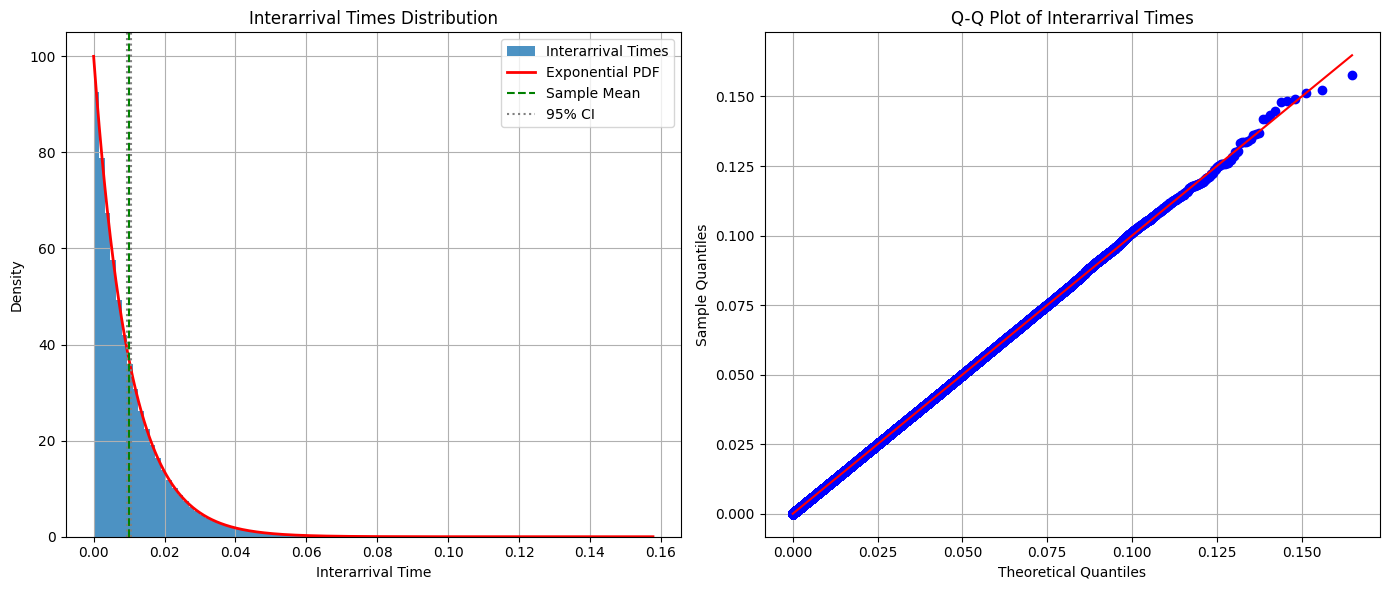
\includegraphics[width=\textwidth]{images/ex1-p1-hl.png}
    \caption{$k = 10^3$ and $\lambda = 100$.}\label{fig:ex1-p1-hl}
  \end{subfigure}
  \caption{Inter-arrival time histograms and Q-Q plots obtained from
  uniform distribution sampling.}\label{fig:ex1-p1-combined}
\end{figure}

\subsection*{Part 2: Exponential Inter-Arrivals}

In this experiment, we generate $k$ realizations of Poisson processes
from $N$ inter-arrival times drawn independently from an exponential
distribution with mean $\frac{1}{\lambda}$.
To sample valid inter-arrival times, we sample $N+1$ inter-arrivals and check the following condition:
\begin{enumerate}
    \setlength\itemsep{0.01em}

  \item That the sum of the first $N$ inter-arrival times does not exceed $T$.
  \item That the sum of all $N+1$ inter-arrival times was greater than $T$.
\end{enumerate}

Condition 2 ensures that there is no bias towards small inter-arrivals.
Arrival times are then
obtained via cumulative summation.

\noindent
We then analyze the resulting arrival times by:

\begin{itemize}
    \setlength\itemsep{0.01em}
  \item Plotting their histogram and overlaying the theoretical
    uniform PDF on $[0, T]$, as illustrated in Figure~\ref{fig:ex1-p2-combined}.
  \item Generating a Q-Q plot to compare the empirical distribution
    with the theoretical uniform distribution.
  \item Computing the empirical mean and variance of the aggregated
    arrival times and assessing their agreement with uniformity assumptions. (Table~\ref{tab:ex1-p2-ci-summary}).
\end{itemize}

\begin{table}[htbp]
  \centering
  \small
  \begin{tabular}{@{}cc|lcccccc@{}}
    \toprule
    $\lambda$ & $k$ & Source & Mean & Var & Mean 95\% CI & Mean 99\%
    CI & Var 95\% CI & Var 99\% CI \\
    \midrule
    100 & $10^3$ & Theoretical & 50.00 & 833.33 & -- & -- & -- & -- \\
    100 & $10^3$ & Empirical   & 50.00 & 833.12 & [48.17,51.75] &
    [47.64,52.22] & [783.70,880.25] & [763.66,907.33] \\
    \midrule
    0.42 & $10^6$ & Theoretical & 50.00 & 833.33 & -- & -- & -- & -- \\
    0.42 & $10^6$ & Empirical   & 50.01 & 833.37 & [49.95,50.06] &
    [49.93,50.08] & [831.91,834.74] & [831.52,835.37] \\
    \bottomrule
  \end{tabular}
  \caption{Summary of arrival time statistics: mean, variance, and
    confidence intervals for both experimental
  setups.}\label{tab:ex1-p2-ci-summary}
\end{table}

\begin{figure}[htbp]
  \centering
  \begin{subfigure}[b]{0.48\textwidth}
    \centering
    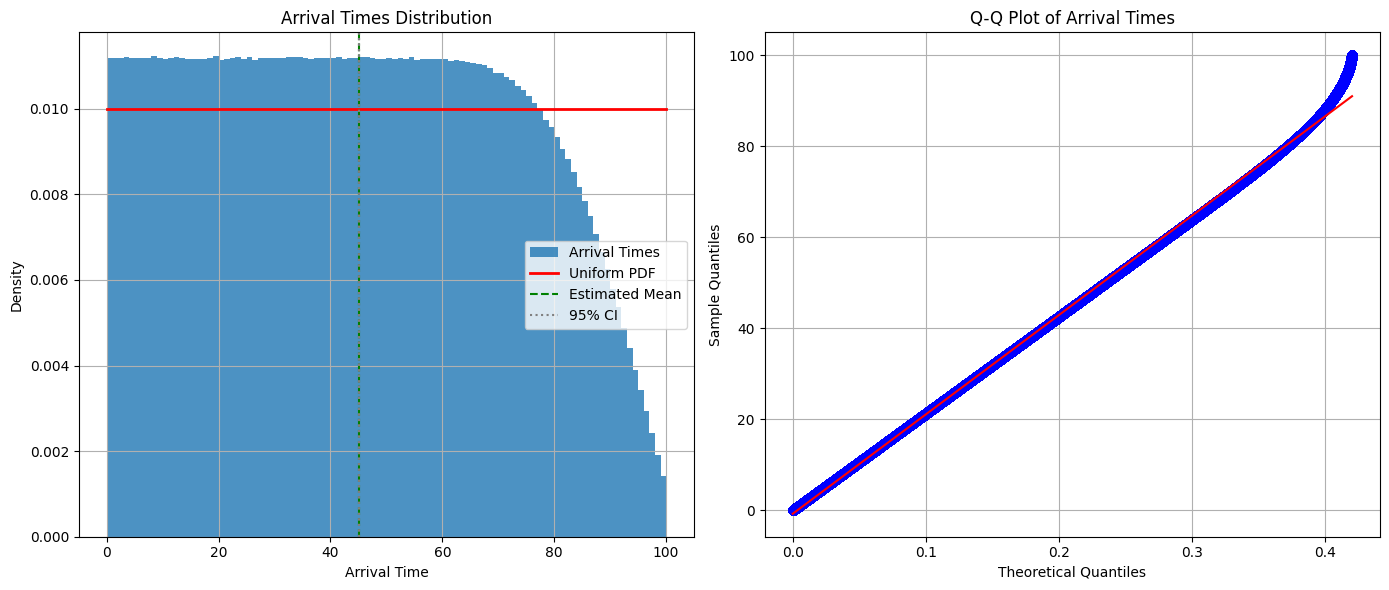
\includegraphics[width=\textwidth]{images/ex1-p2.png}
    \caption{$k = 10^6$ and $\lambda = 0,42$.}\label{fig:ex1-p2}
  \end{subfigure}
  \hfill
  \begin{subfigure}[b]{0.48\textwidth}
    \centering
    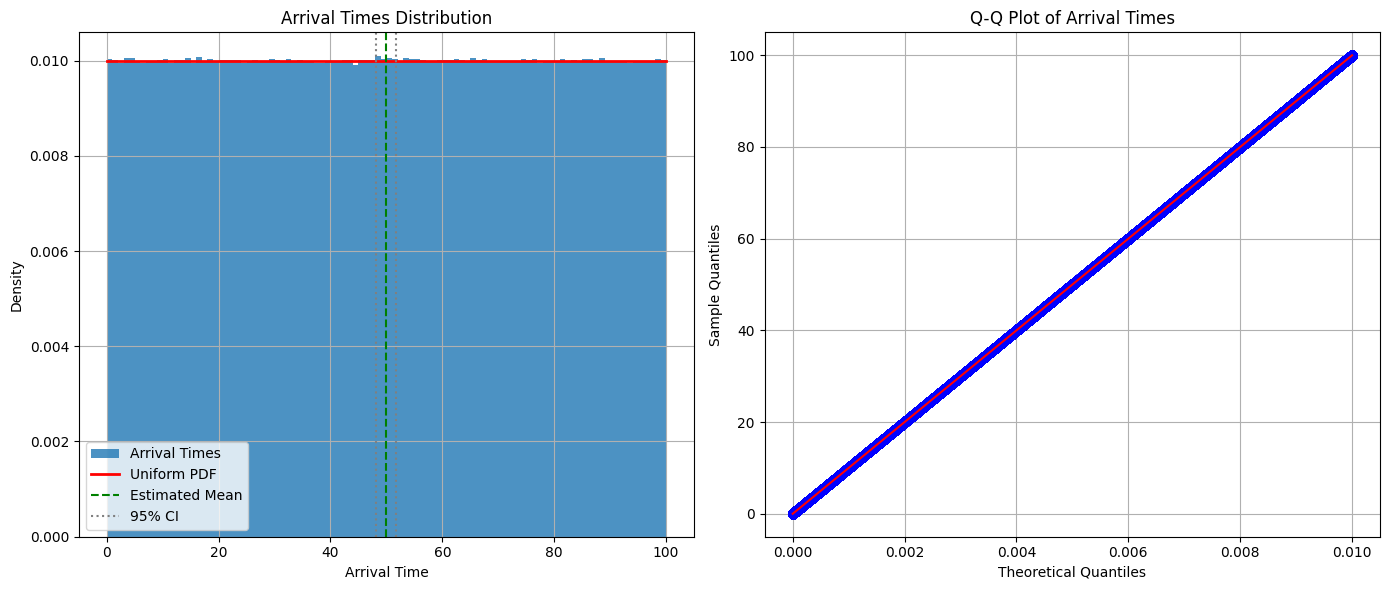
\includegraphics[width=\textwidth]{images/ex1-p2-hl.png}
    \caption{$k = 10^3$ and $\lambda = 100$.}\label{fig:ex1-p2-hl}
  \end{subfigure}
  \caption{Arrival time histograms and Q-Q plots obtained from
  exponential inter-arrival times..}\label{fig:ex1-p2-combined}
\end{figure}

\section*{Exercise 2}

\subsection*{Rejection Sampling}
To apply the rejection sampling, we need to find a distribution such
that we can bound the probability $f(x)$ such that
\begin{equation*}
  \frac{f(x)}{g(x)} \leq c
\end{equation*}

A valid proposal distribution can be
\begin{equation*}
  g(x) =
  \begin{cases}
    k \, x^2 \quad \text{if} \quad -3\leq x\leq3 \\
    0 \quad \text{otherwise}
  \end{cases}
\end{equation*}
where $k$ is such that $\int_{-3}^{3} g(x) \, dx =1$.
Such $k$ is given by
\begin{equation*}
  \int_{-3}^{3} g(x) \, dx =\int_{-3}^{3} kx^2 \, dx =  18k
  \overset{!}{=} 1 \Rightarrow k = \frac{1}{18}
\end{equation*}

The proposal distribution is then $g(x) = \frac{x^2}{18}$ and the bound is
\begin{equation}
  \label{eq:c}
  \frac{\frac{1}{A}x^2\sin^2(\pi x)}{\frac{x^2}{18}} =
  \frac{18}{A}\sin^2(\pi x) \leq c \Rightarrow c = \frac{18}{A} = 2.03435386.
\end{equation}
To draw a sample from the distribution $g(x)$ we can apply the
CDF-Inversion method, so we derive the inverse of the CDF $G(x)$:

\begin{equation*}
  G(x) = \int_{-3}^{x}g(t)\,dt = \int_{-3}^{x} \frac{t^2}{18}\,dt =
  \frac{1}{2}+\frac{x^3}{54}
  \Rightarrow G^{-1}(u) = 3\sqrt[3]{2(u-\frac{1}{2})} \quad
  \text{for}\quad u \in [0,1].
\end{equation*}

We can now choose 2 ways of applying the rejection sampling, the
first with the knowledge of A, which allow us to have an higher
acceptance rate, or without knowledge of A, which allow us to know
the target distribution up to a constant but it does not let us to
bound it so tightly, having a drop in the acceptance rate. We report
both methods in the following.

\subsubsection*{Algorithm with the full knowledge of $f(x)$}
In this case we assume to know the value of $A$, so that we know also
the value of $c$ from\ref{eq:c}, so we can bound $f(x)$ with the
function $cg(x) = \frac{18}{A}\frac{x^2}{18} =\frac{x^2}{A}$ which is
basically the envelope of $f(x)$.
Thus, the algorithm is the one reported in Algorithm\ref{alg:1}.

\begin{algorithm}
  \caption{Rejection sampling with full knowledge of $f(x)$}\label{alg:1}
  \begin{algorithmic}[1]
    \STATE~Draw $u_1 \sim \mathcal{U}[0,1]$
    \STATE~Compute $x = G^{-1}(u_1)$
    \STATE~Draw $u_2 \sim \mathcal{U}[0, c \cdot g(x)]$
    \IF{$u_2 < f(x)$}
    \STATE~Accept $x$
    \ELSE%
    \STATE~Go back to Step 1
    \ENDIF%
  \end{algorithmic}
\end{algorithm}

The distribution resulting from Algorithm~\ref{alg:1} is shown in
Figure~\ref{fig:rej-sik}. The acceptance rate of this algorithm in
$10^8$ iterations is $\frac{10^8}{49155544} \approx 0.49$. The
distribution of the drawn samples is shown against the theoretical
one in Figure~\ref{fig:rej-sik}, while the accepted samples and the
rejected samples (from the proposal) are shown in~\ref{fig:rs-sik}.

\subsubsection*{Algorithm with knowledge of $f(x)$ up to a constant}
Given that $f(x) = \frac{1}{A}x^2\sin^2(\pi x)=\frac{1}{A}f^n(x)$, if
we do not know the value of A, we can still bound the non-normalized
distribution $f^{n}(x)$:
\begin{equation}
  f^n(x) = x^2\sin^2(\pi x) \leq x^2 \leq 9 = M\quad \text{in}\quad
  -3\leq x\leq3
\end{equation}
We can use this upper bound do apply rejection sampling as in
Algorithm~\ref{alg:2}.

\begin{algorithm}
  \caption{Rejection sampling with knowledge of $f(x)$ up to a
  constant}\label{alg:2}
  \begin{algorithmic}[1]
    \STATE~Draw $x \sim \mathcal{U}[-3,3]$
    \STATE~Draw $u \sim \mathcal{U}[0, M]$
    \IF{$u \leq f^n(x)$}
    \STATE~Accept $x$
    \ELSE%
    \STATE~Go back to Step 1
    \ENDIF%
  \end{algorithmic}
\end{algorithm}

We see that in this algorithm we do not employ $A$ at all, and the
proposal distribution is a uniform distribution. We build a
``bounding box'' around the scaled distribution $f^n(x)$ and accept
only those points that fall under the plot of $f^n(x)$. This approach
works, but, clearly, being less precise in the bounding, the
acceptance rate drops: the acceptance rate on $10^8$ iterations is
$\frac{10^8}{16381697} \approx 0.16$. The distribution of the drawn
samples is shown against the theoretical one in
Figure~\ref{fig:rej-nok},, while the accepted samples and the
rejected samples (from the proposal) are shown in Figure~\ref{fig:rs-nok}.

\subsection*{Confidence intervals}
For the computation of the confidence intervals, since the data are
i.i.d., we use the order statistics and the binomial distribution
(approximated with a normal, since $n=200$ is large enough) for the
CIs of the median and the 0.9-quantile.
For a quantile $q$, the formula for CI $[X_{(j)},X_{(k)}]$ is (using
the normal approximation of the binomial):

\begin{equation*}
  j \approx \lfloor nq-1.96\sqrt{nq(q-q)} \rfloor, \quad k \approx
  \lfloor nq+1.96\sqrt{nq(q-q)} \rfloor +1.
\end{equation*}

Instead, for the mean, we exploit the central limit Theorem (since we
have enough data points and the distribution is symmetric) and obtain
the confidence interval:
\begin{equation*}
  \hat{\mu_n} \pm \eta\frac{s_n}{\sqrt{n}}
\end{equation*}

For the bootstrap procedure, the only assumption is to have
i.i.d.\ data, so we can also apply it.

The plots of the median and the 0.9-quantile computed with the two
different approaches are shown in Figure~\ref{fig:med-Q}.

The plots for the mean are shown in Figure~\ref{fig:mean-CI}.

\subsubsection*{Statistical significance of the mean's confidence intervals}

We subdivided 20000 variates into 100 disjoint sets and for each of
them we computed the 95\% confidence intervals, both with the
Gaussian approximation approach and the Bootstrap approach. As
expected, the number of confidence intervals containing the true mean
is 95 in the case of the Gaussian approximation and 94 in the case of
the bootstrap CIs (we can see that the bootstrap method slightly
understimates the CI, so we find less accurate CIs).
Figure~\ref{fig:CLT} shows the distribution of the sample mean
computed in the 100 sets, showing that the Central Limit Theorem
holds over this statistic.

\begin{figure}[htbp]
  \centering
  \begin{subfigure}[b]{0.45\textwidth}
    \centering
    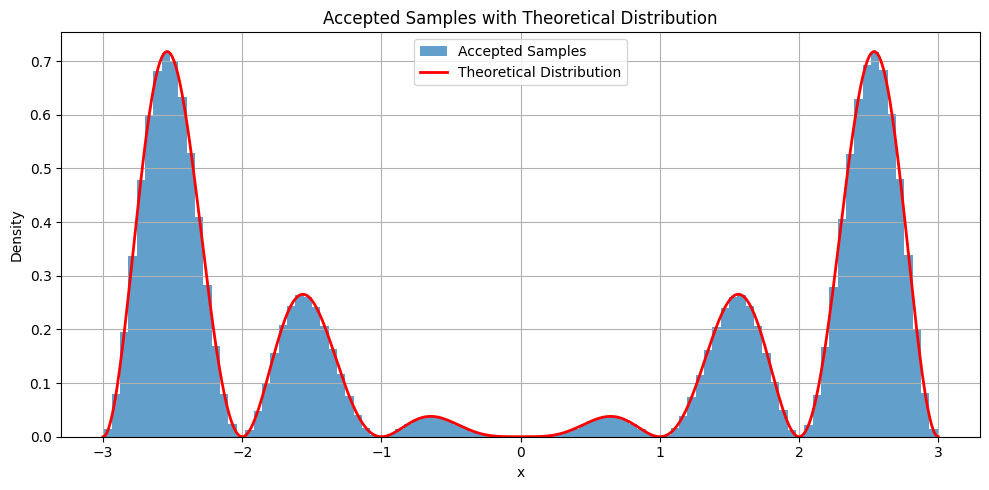
\includegraphics[width=\textwidth]{images/rej-sampl-SIK.png}
    \caption{Rejection sampling with Algorithm~\ref{alg:1}.}\label{fig:rej-sik}
  \end{subfigure}\hfill
  \begin{subfigure}[b]{0.45\textwidth}
    \centering
    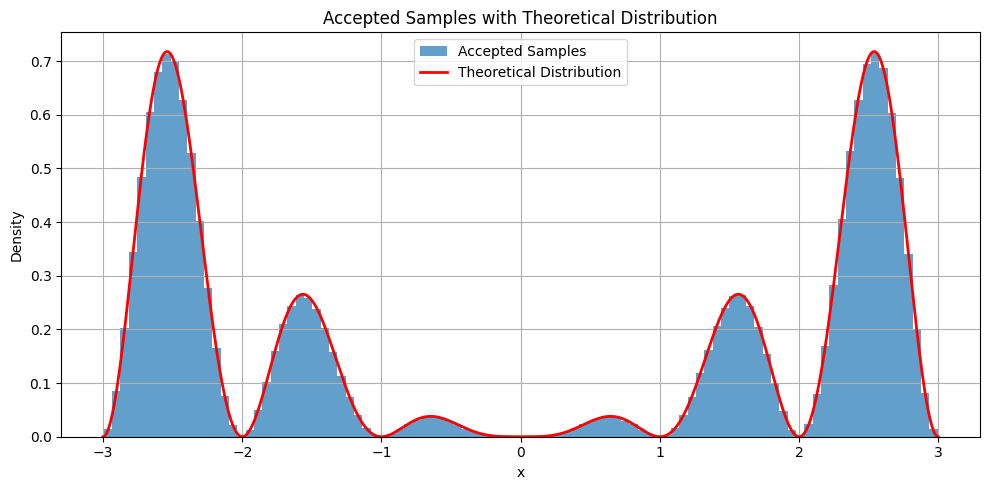
\includegraphics[width=\textwidth]{images/rej-sampl-NOK.png}
    \caption{Rejection sampling with Algorithm~\ref{alg:2}.}\label{fig:rej-nok}
  \end{subfigure}\label{fig:rej-sampl}
  \caption{Rejection sampling of $f(x)$}
\end{figure}

\begin{figure}[htbp]
  \centering
  \begin{subfigure}[b]{0.45\textwidth}
    \centering
    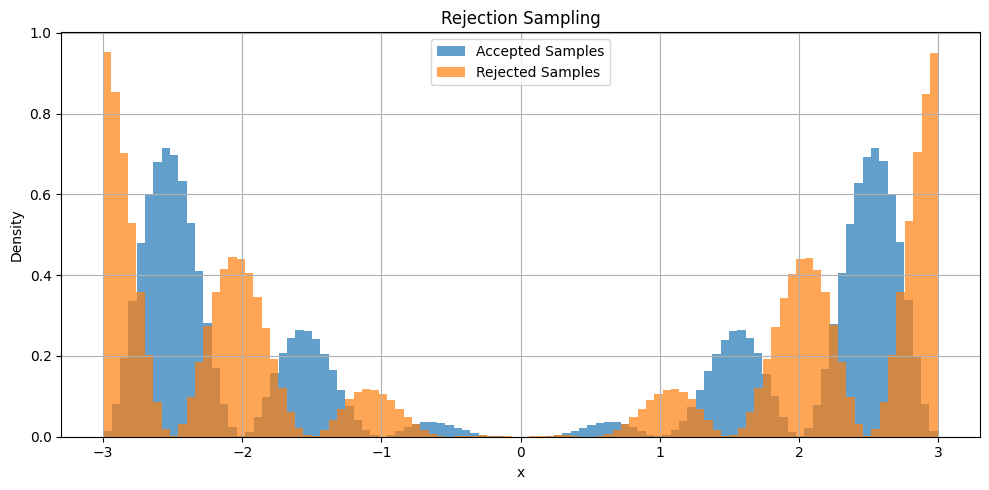
\includegraphics[width=\textwidth]{images/rs-acc-rej_SIK.png}
    \caption{Rejected/accepted samples with
    Algorithm~\ref{alg:1}.}\label{fig:rs-sik}
  \end{subfigure}
  \hfill
  \begin{subfigure}[b]{0.45\textwidth}
    \centering
    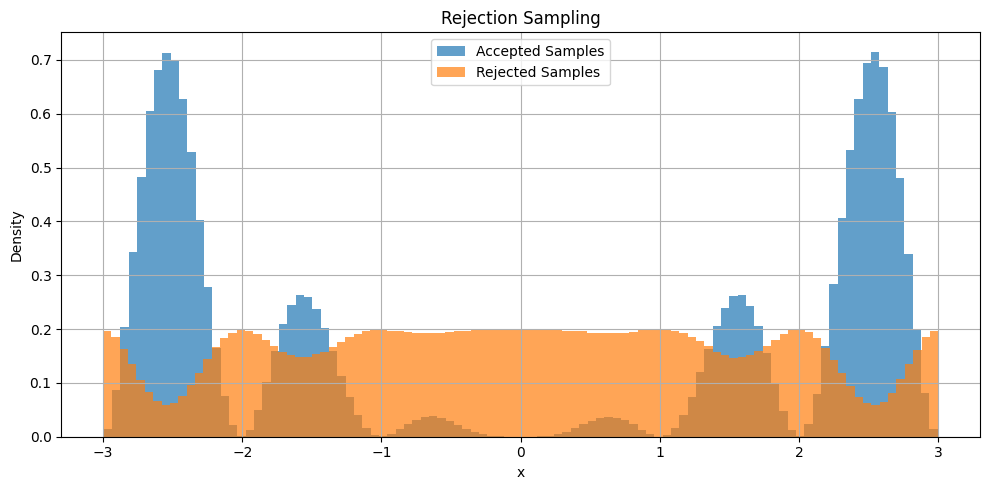
\includegraphics[width=\textwidth]{images/rs-acc-rej_NOK.png}
    \caption{Rejected/accepted samples with
    Algorithm~\ref{alg:2}.}\label{fig:rs-nok}
  \end{subfigure}\label{fig:rej-sampl2}
  \caption{Accepted/rejected samples distributions.}
\end{figure}

\begin{figure}[htbp]
  \centering
  \begin{subfigure}[b]{0.45\textwidth}
    \centering
    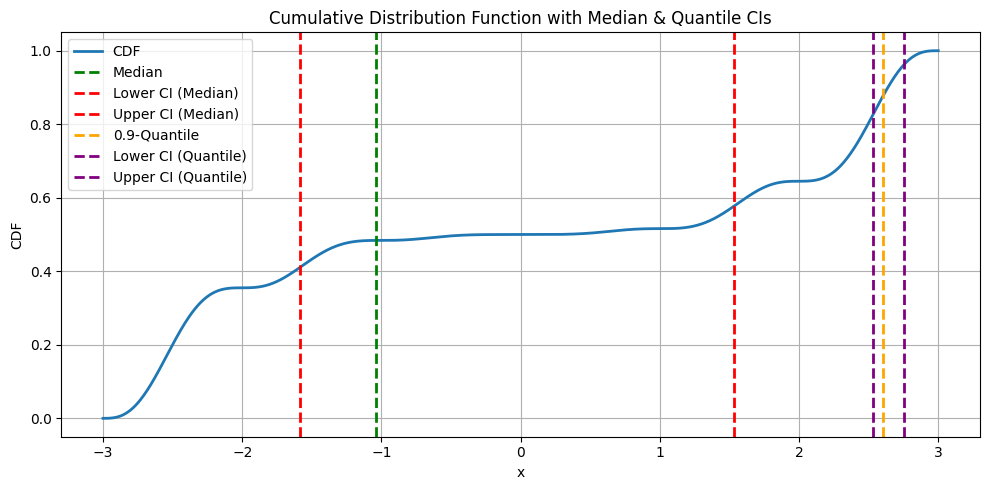
\includegraphics[width=\textwidth]{images/med-Q-CI.png}
    \caption{Median and 0.9-Quantile CIs computed with the Binomial
    formula.}\label{fig:med-Q-1}
  \end{subfigure}
  \hfill
  \begin{subfigure}[b]{0.45\textwidth}
    \centering
    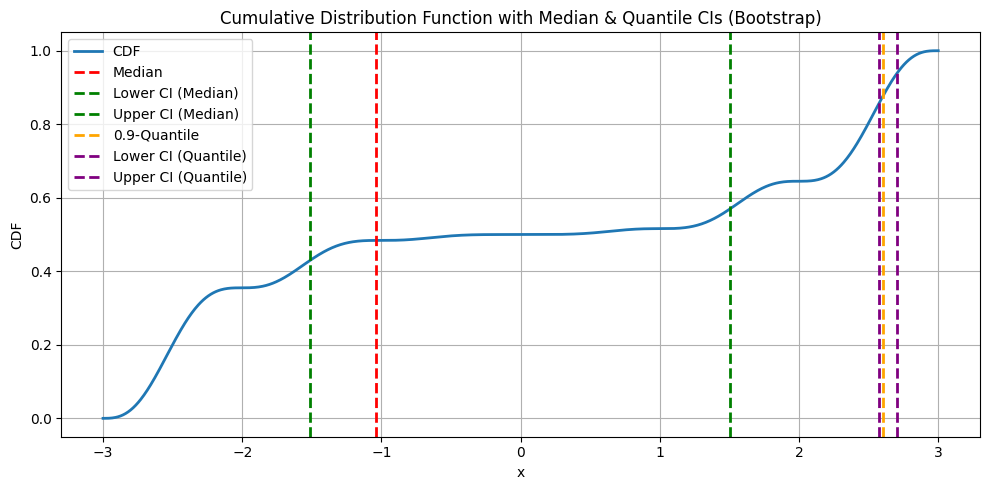
\includegraphics[width=\textwidth]{images/med-Q-Boot-CI.png}
    \caption{Median and 0.9-Quantile CIs computed with the Bootstrap
    heuristic.}\label{fig:med-Q-2}
  \end{subfigure}
  \caption{CDF with median and 0.9-quantile CIs.}\label{fig:med-Q}
\end{figure}

\begin{figure}[htbp]
  \centering
  \begin{subfigure}[b]{0.45\textwidth}
    \centering
    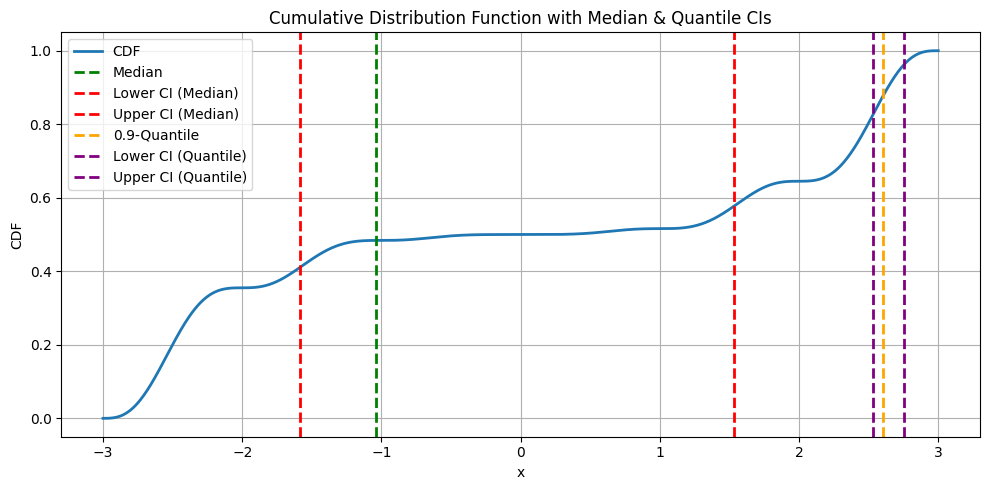
\includegraphics[width=\textwidth]{images/med-Q-CI.png}
    \caption{Mean CI computed with the Gaussian
    approximation.}\label{fig:mean-1}
  \end{subfigure}
  \hfill
  \begin{subfigure}[b]{0.45\textwidth}
    \centering
    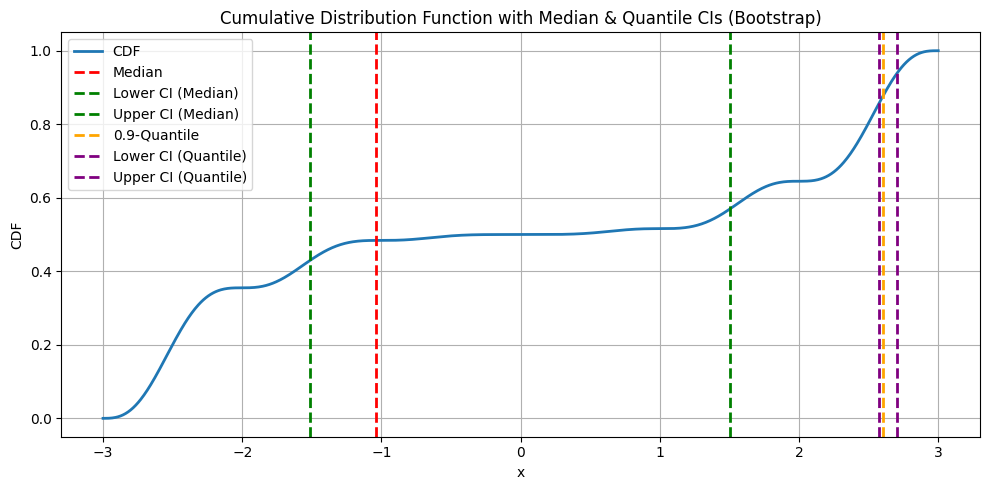
\includegraphics[width=\textwidth]{images/med-Q-Boot-CI.png}
    \caption{Mean CI computed with the Bootstrap heuristic.}\label{fig:mean-2}
  \end{subfigure}
  \caption{PDF and mean CI.}\label{fig:mean-CI}
\end{figure}

\begin{figure}[htbp]
  \centering
  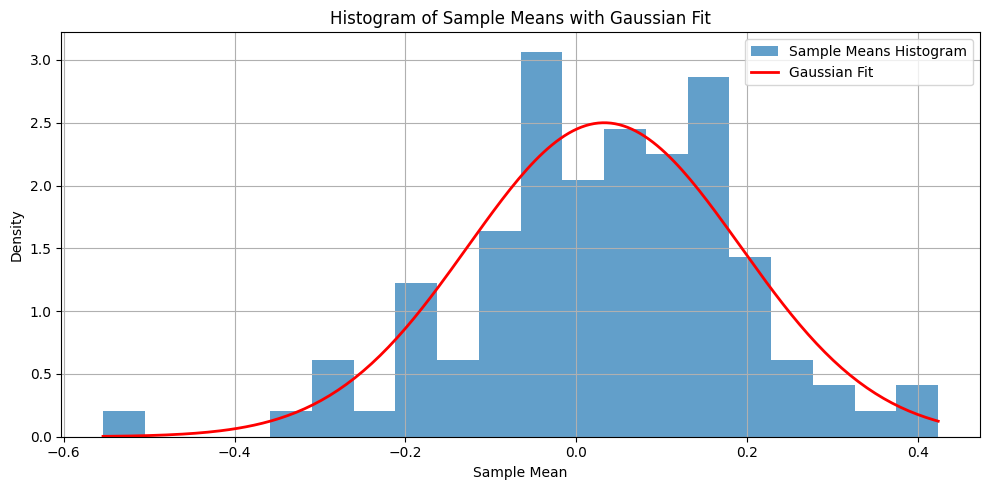
\includegraphics[width=0.8\textwidth]{images/CLT3.png}
  \caption{Empirical PDF of the sample mean.}\label{fig:CLT}
\end{figure}

\end{document}
